
\boxde
\Opensolutionfile{ans}[ans/2D1-5-DEON-2]
\begin{ex}%[2D1B5-1]
    \immini{Bảng biến thiên ở hình bên là của hàm số nào trong các hàm số dưới đây?
        \choice
        {$y=-x^3+3x^2-3$}
        {$y=x^3+3x^2-1$}
        {$y=x^3-3x+2$}
        {\True $y=x^3-3x^2+2$}}{
\begin{tikzpicture}
            \tkzTabInit[nocadre=false, lgt=1.2, espcl=2.5, deltacl=0.6]{$x$/0.6,$y'$/0.6,$y$/2}
            {$-\infty$, $0$, $2$, $+\infty$}
            \tkzTabLine {,+,0,-,0,+,}
            \tkzTabVar{-/$-\infty$, +/$2$, -/$-2$, +/$+\infty$}
    \end{tikzpicture}}
    \loigiai
    {Hàm số trong $4$ phương án có dạng $y=ax^3+bx^2+cx+d$ với $a\neq 0$.\\
        Theo bảng biến thiên ta có $\lim\limits_{x\to +\infty}y=+\infty$ nên $a>0$.\\
        Tiếp đến, đồ thị đi qua điểm $(0;2)$ nên $d=2$.\\
        Xét hàm số $f(x)=x^3-3x^2+2$ và $g(x)=x^3-3x+2$. Ta có $f(2)=-2$ và $g(2)=4\neq -2$.\\
        Vậy bảng biến thiên đã cho là của hàm số $y=x^3-3x^2+2$.
    }
\end{ex}
\begin{ex}%[2D1B5-3]
    Tất cả giá trị của tham số $m$ đề đồ thị hàm số $(\mathrm{C})\colon y=-2x^3+3x^2+2m-1$ cắt trục hoành tại ba điểm phân biệt là
    \choice
    {$\dfrac{1}{4}\le m< \dfrac{1}{2}$}
    {$-\dfrac{1}{2}<m<\dfrac{1}{2}$}
    {\True $0<m<\dfrac{1}{2}$}
    {$0\le m\le \dfrac{1}{2}$}
    \loigiai{Phương trình hoành độ giao điểm
        $$-2x^3+3x^2+2m-1=0\Leftrightarrow 2m=2x^3-3x^2+1.$$
        Xét $g(x)=2x^3-3x^2+1$, $\mathscr{D}=\mathbb{R}$.\\
        $g'(x)=6x^2-6x$, $g'(x)=0\Leftrightarrow \hoac{&x=0\\&x=1.}$\\
        Bảng biến thiên \\
        \begin{center}
            
\begin{tikzpicture}[>=stealth]
                \tkzTabInit[nocadre=false,lgt=1.2,espcl=2.2,deltacl=0.5]{$x$/.7 ,$g'(x)$/.7,$g(x)$/2.1}
                {$-\infty$ , $0$ , $1$ , $+\infty$}
                \tkzTabLine{ , + , $0$ , - , $0$ , + , }
                \tkzTabVar{-/$-\infty$ , +/$1$ , -/$0$ , +/$+\infty$}
            \end{tikzpicture}
        \end{center}
        $(\mathrm{C})$ cắt trục hoành tại $3$ điểm phân biệt \\
        $\Leftrightarrow$ đường thẳng $d\colon y=2m$ cắt đường cong $(\mathrm{C_1})\colon g(x)=2x^3-3x^2+1$ tại $3$ điểm phân biệt\\
        $\Leftrightarrow 0<2m<1\Leftrightarrow 0<m<\dfrac{1}{2}.$
    }
\end{ex}
\begin{ex}%[2D1B5-4]
    Tìm tất cả các giá trị thực của tham số $m$ để đường thẳng $y=m$ cắt đồ thị hàm số $y=x^4-2x^2$ tại $4$ điểm phân biệt.
    \choice
    {\True $-1<m<0$}
    {$m<0$}
    {$0<m<1$}
    {$m>0$}
    \loigiai{
        Tập xác định $\mathscr{D}=\mathbb{R}$.\\
        $y'=4x^3-4x$, $y'=0\Leftrightarrow\hoac{&x=0\Rightarrow y=0\\&x=\pm 1\Rightarrow y=-1.}$ \\
        Bảng biến thiên
        \begin{center}
            
\begin{tikzpicture}
                \tkzTabInit[espcl=2.3,lgt=1.3]
                {$x$/0.7,$y'$/0.7,$y$/2.1}
                {$-\infty$,$-1$,0,$1$,$+\infty$}
                \tkzTabLine{,+,0,-,0,+,0,-}
                \tkzTabVar{-/$-\infty$,+/$-1$,-/$0$,+/$-1$,-/$-\infty$}
            \end{tikzpicture}
        \end{center}
        Dựa vào bảng biến thiên ta có giá trị $m$ cần tìm là $-1<m<0$.}
\end{ex}
\begin{ex}%[2D1B5-3]
    \immini{Cho hàm số $y=f(x)=ax^4+bx^2+c$ có đồ thị như hình vẽ. Số nghiệm của phương trình $2f(x)+3=0$ là
        \choice
        {$ 3 $}
        {$ 1 $}
        {$ 2 $}
        {\True $ 4 $}
    }{
        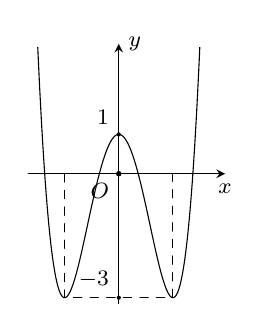
\begin{tikzpicture}[scale=0.5, font=\footnotesize,line join=round, line cap=round,>=stealth]
            \draw[->] (-2.3,0.) -- (2.7,0.) node[below]{$x$};
            \draw[->] (0,-3.3) -- (0,3.3) node[right]{$y$};
            \clip (-2.3,-3.3) rectangle (2.7,3.2);
            \fill (0,0) circle(2pt) node[below left]{$O$};
            \fill (0,-3.148405224) circle(1.5pt) node[above left]{$-3$};
            \fill (0,1) circle(1.5pt) node[above left]{$1$};
            \draw[smooth,samples=300,domain=-2.1:2.1] plot(\x,{(73/63)*(\x)^4-(1105/252)*(\x)^2+1});
            \draw [dashed] (-1.375544724,0) -- (-1.375544724,-3.148405224) -- (1.375544724,-3.148405224) -- (1.375544724,0);
        \end{tikzpicture}
    }
    \loigiai{
        Ta có $2f(x)+3=0 \Leftrightarrow f(x)=-\dfrac{3}{2}$. Đây là phương trình hoành độ giao điểm của đồ thị hàm số đã cho và đường thẳng $\Delta \colon y=-\dfrac{3}{2}$.
        Dựa vào đồ thị thì hàm số có cực đại là $y_{\text{CĐ}}=1$ và cực tiểu là $y_{\text{CT}}=-3$.
        Mà $-3<-\dfrac{3}{2}<1$ nên đường thẳng $\Delta$ cắt đồ thị đã cho tại $4$ điểm.\\
        Vậy phương trình $2f(x)+3=0$ có $4$ nghiệm.
    }
\end{ex}
\begin{ex}%[2D1Y5-1]
    \immini{Đường cong trong hình bên là đồ thị của một hàm số trong bốn hàm số được liệt kê ở bốn phương án $A$, $B$, $C$, $D$ dưới đây. Hỏi hàm số đó là hàm số nào?
        \choice
        {$y=-x^2+x-1$}
        {$y=-x^3+3x+1$}
        {\True $y=x^3-3x+1$}
        {$y=x^4-x^2+1$}}{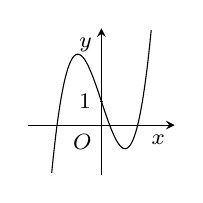
\begin{tikzpicture}[scale=0.3, font=\footnotesize, line join=round, line cap=round, >=stealth]
            \draw[->] (-3.1,0)--(3.1,0) node[below left] {$x$};
            \draw[->] (0,-2.1)--(0,4.1) node[below left] {$y$};
            \draw (0,0) node [below left] {$O$};
            \foreach \y in {1}
            \draw[thin] (1pt,\y)--(-1pt,\y) node [left] {$\y$};
            \begin{scope}
                \clip (-3,-2) rectangle (3,4);
                \draw[samples=200,domain=-3:3,smooth,variable=\x] plot (\x,{1*((\x)^3)+0*((\x)^2)+-3*(\x)+1});
            \end{scope}
            % \begin{scope}[on background layer]\path[white]node{MDD-108};\end{scope}
    \end{tikzpicture}}
    \loigiai{
        Đồ thị hàm số là đồ thị hàm bậc ba $y=ax^3+bx^2+cx+d$.\\
        Ta thấy $\lim\limits_{x \to +\infty} y = +\infty$ nên $a>0$.
    }
\end{ex}
\begin{ex}%[2D1B5-3]
    Số giao điểm của đồ thị hàm số $y=(x^2-1)(2-x^2)$ với trục hoành là
    \choice
    {\True $4$}
    {$2$}
    {$3$}
    {$0$}
    \loigiai{
        Phương trình hoành độ giao điểm của đồ thị hàm số $y=(x^2-1)(2-x^2)$ với trục hoành là
        $$(x^2-1)(2-x^2)=0 \Leftrightarrow \hoac{& x^2=1 \\ & x^2=2} \Leftrightarrow \hoac{& x=\pm 1 \\ & x= \pm \sqrt{2}.}$$
        Vậy số giao điểm của đồ thị hàm số đã cho với trục hoành là $4$.
    }
\end{ex}
\begin{ex}%[2D1Y5-1]
    \immini{	Đường cong ở hình bên là đồ thị của hàm số $y=ax^4+bx^2+c$. Mệnh đề nào sau đây đúng?
        \choice
        {$y'=0$ có hai nghiệm và $a<0$}
        {$y'=0$ có ba nghiệm và $a>0$}
        {$y'=0$ có hai nghiệm và $a>0$}
        {\True $y'=0$ có một nghiệm và $a<0$}}{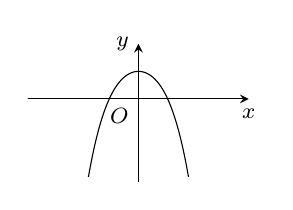
\begin{tikzpicture}[scale=0.7,>=stealth, font=\footnotesize, line join=round, line cap=round]
            \def\a{-1} \def\b{-1.5} \def\c{0.5} % Hệ số
            \def\xmin{-2} \def\xmax{2}
            \def\ymin{-1.5} \def\ymax{1}
            %	\draw[color=gray!50,dashed] (\xmin,\ymin) grid (\xmax,\ymax);
            \draw[->] (\xmin,0)--(\xmax,0) node [below]{$x$};
            \draw[->] (0,\ymin)--(0,\ymax) node [left]{$y$};
            \node at (0,0) [below left]{$O$};
            \clip (\xmin+0.1,\ymin+0.1) rectangle (\xmax-0.5,\ymax-0.1);
            \draw[smooth,samples=300,domain=-2:2.5] plot(\x,{\a*(\x)^4+\b*(\x)^2+\c});
    \end{tikzpicture}}
    \loigiai{
        Dựa vào đồ thị ta có $y'=0$ có một nghiệm và $a<0$.
    }
\end{ex}
\begin{ex}%[2D1B5-3]
    Cho hàm số $y=f(x)$ có bảng biến thiên như hình vẽ.
    \begin{center}
        
\begin{tikzpicture}
            \tkzTabInit[nocadre,espcl=2.5,lgt=1.5]
            {$x$/0.6,$y'$/0.6,$y$/2.2}
            {$-\infty$,$-2$,$3$,$+\infty$}
            \tkzTabLine{,+,d,-,d,+,}
            \tkzTabVar{-/$-\infty$,+/$2$,-/$1$,+/$+\infty$}\end{tikzpicture}
        \par\end{center}
    Số nghiệm thực của phương trình $2f(x)-3=0$ là
    \choice {$2$}{$1$} {\True $3$ } {$4$ }
    \loigiai{Ta có $2f(x)-3=0\Leftrightarrow f(x)=\dfrac{3}{2}.$
        $\hfill(*)$ \\
        Số nghiệm phương trình ({*}) là số giao điểm của đồ thị hàm số $y=f(x)$
        và đường thẳng $y=\dfrac{3}{2}$. \\
        Bảng biến thiên.
        \begin{center}
            \begin{tikzpicture}
                \tkzTabInit[nocadre,espcl=2.5,lgt=1.5]
                {$x$/0.6,$y'$/0.6,$y$/2.2}
                {$-\infty$,$-2$,$3$,$+\infty$}
                \tkzTabLine{,+,d,-,d,+,}
                \tkzTabVar{-/$-\infty$,+/$2$,-/$1$,+/$+\infty$}
                \draw [color=blue] ($(N13)!0.5!(N12) $) -- ($ (N42)!0.5!(N43) $) node [below] {$ y=\dfrac{3}{2} $};
            \end{tikzpicture}
            \par\end{center}
        \noindent Dựa vào bảng biến thiên ta được phương trình $f(x)=\dfrac{3}{2}$
        có ba nghiệm phân biệt.
} \end{ex}
\begin{ex}%[2D1B5-3]
    Cho hàm số $y=f(x)$ có bảng biến thiên như sau. Số nghiệm phương trình $f(x)-2=0$ là\\
    \centerline{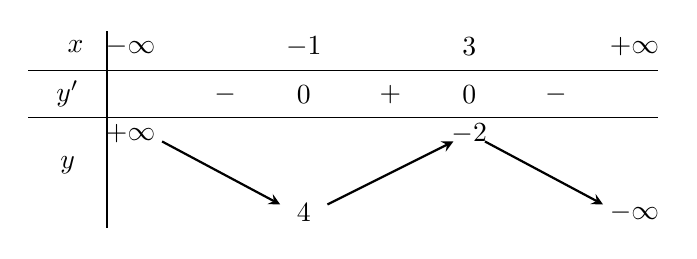
\begin{tikzpicture}[>=stealth,scale=1]
            %\draw[ultra thin,gray!20](-1.1,-2.1) grid (7.1,0.6);
            \draw (-1.,0.)-- (7.,0.);
            \draw (-1.,-0.6)-- (7.0,-0.6);
            \draw (0.,0.5)-- (0.,-2.);
            \draw (-0.4,0.3) node {$x$};
            \draw (0.3,0.3) node {$-\infty$};
            \draw (6.7,0.3) node {$+\infty$};
            \draw (2.5,0.3) node {$-1$};
            \draw (4.6,0.3) node {$3$};
            \draw (-0.5,-0.3) node {$y'$};
            \draw (2.5,-0.3) node {$0$};
            \draw (4.6,-0.3) node {$0$};
            \draw (1.5,-0.3) node {$-$};
            \draw (3.6,-0.3) node {$+$};
            \draw (5.7,-0.3) node {$-$};
            \draw (-0.5,-1.2) node {$y$};
            \draw (2.5,-1.8) node {$4$};
            \draw (4.6,-0.8) node {$-2$};
            \draw (0.3,-0.8) node {$+\infty$};
            \draw (6.7,-1.8) node {$-\infty$};
            \draw [->,thick] (0.7,-0.9) -- (2.2,-1.7);
            \draw [->,thick] (2.8,-1.7) -- (4.4,-0.9);
            \draw [->,thick] (4.8,-0.9) -- (6.3,-1.7);
    \end{tikzpicture}}
    \choice
    {$0$}
    {\True $3$}
    {$1$}
    {$2$}
    \loigiai{
        Số nghiệm của phương trình $f\left( x \right) - 2 = 0 \Leftrightarrow f\left( x \right) = 2$ là số giao điểm của đồ thị hàm số $y = f\left( x \right)$ và đường thẳng $y = 2$
        Theo BBT ta thấy đường thẳng $y = 2$ cắt đồ thị hàm số $y = f\left( x \right)$ tại 3 điểm phân biệt.
    }
\end{ex}
\begin{ex}%[2D1B5-4]
    \immini{Cho hàm số $y=f(x)$ có đồ thị như hình vẽ bên. Phương trình $f(x)=-3$ có số nghiệm là
        \choice
        {$0$}
        {$1$}
        {$2$}
        {\True $3$}}
    {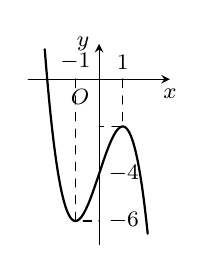
\begin{tikzpicture}[>=stealth,line join=round,line cap=round,font=\footnotesize,scale=0.3]
            \def\a{-1} \def\b{0} \def\c{3} \def\d{-4}% Hệ số
            \draw[->] (-3,0)--(3,0) node[below]{$x$};
            \draw[->] (0,-7)--(0,1.5) node[left]{$y$};
            \fill[name=O] (0,0) circle (1pt) node[below left] {$O$};
            \draw[color=black,thick, smooth, samples=200, domain= -2.3:2.06] plot(\x,{\a*(\x)^3+\b*(\x)^2+\c*(\x)+\d});
            \draw[dashed] (1,0)|-(0,-2) (-1,0)|-(0,-6);
            \foreach \x in {-1,1}
            \fill (\x,0)node[above]{$\x$} circle (1pt);
            \foreach \y in {-6,-4}
            \fill (0,\y)node[right]{$\y$} circle (1pt);
    \end{tikzpicture}}
    \loigiai{
        Dựa vào đồ thị, đường thẳng $y=-3$ cắt đồ thị tại $3$ điểm nên phương trình $f(x)=-3$ có $3$ nghiệm phân biệt.}
\end{ex}
\begin{ex}%[2D1B5-3]
    Cho hàm số $y=f(x)$ có bảng biến thiên như hình vẽ sau
    \begin{center}
        
\begin{tikzpicture}
            \tkzTabInit[nocadre=false,lgt=1.2,espcl=2.5,deltacl=0.6]
            {$x$ /0.6,$y'$ /0.6,$y$ /2}
            {$-\infty$,$-1$,$0$,$1$,$+\infty$}
            \tkzTabLine{,-,$0$,+,$0$,-,$0$,+,}
            \tkzTabVar{+/$+\infty$, -/$1$,+/$2$,-/$1$,+/$+\infty$}
            % \begin{scope}[on background layer]\path[white]node{MDD-109};\end{scope}
        \end{tikzpicture}
    \end{center}
    Tìm tất cả các giá trị thực của tham số $m$ để phương trình $f(x)-m=0$ có $4$ nghiệm phân biệt.
    \choice
    {$m\in [-1;2]$}
    {\True $m\in (1;2)$}
    {$m\in (1;2]$}
    {$m \in [1;2)$}
    \loigiai{
        Ta có $f(x)-m=0 \Leftrightarrow f(x)=m$. Phương trình có $4$ nghiệm khi và chỉ khi đường thẳng $y=m$ cắt đồ thị hàm số $y=f(x)$ tại $4$ điểm. Suy ra $m \in (1;2)$.
    }
\end{ex}
\begin{ex}%[2D1Y5-1]
    Bảng biến thiên sau đây là bảng biến thiên của hàm số nào?
    \begin{center}
        
\begin{tikzpicture}[>=stealth]
            \tkzTabInit[nocadre=false,lgt=1,espcl=2.5,deltacl=0.5]{$x$/.7 ,$y'$/.7,$y$/2}
            {$-\infty$ , $0$ , $2$ , $+\infty$}
            \tkzTabLine{ , - , $0$ , + , $0$ , - , }
            \tkzTabVar{+/$+\infty$ , -/$-1$ , +/$3$ , -/$-\infty$}
        \end{tikzpicture}
    \end{center}
    \choice
    {$y=x^3+3x^2-1$}
    {$y=x^3-3x^2-1$}
    {$y=-x^3-3x^2-1$}
    {\True $y=-x^3+3x^2-1$}
    \loigiai{
        Dựa vào bảng biến thi ta có các nhận xét.
        \begin{itemize}
            \item Nhánh ngoài cùng đi xuống suy ra hệ số $a<0$.
            \item $y'=0\Leftrightarrow \hoac{& x=0 \\& x=2}$
        \end{itemize}
    }
\end{ex}
\begin{ex}%[2D1K5-1]
    \immini{Cho hàm số $ f(x)=ax^4+bx^2+c $ ($ a\ne 0 $) có đồ thị như hình vẽ.
        Tìm mệnh đề đúng trong các mệnh đề sau.
        \choice
        { $ a>0, b<0, c>0 $ }
        { $ a<0, b>0, c<0 $ }
        { $ a<0, b<0, c>0 $ }
        {\True $ a<0, b>0, c>0 $ }}
    {\begin{tikzpicture}[>=stealth,line join=round,line cap=round,font=\footnotesize,scale=0.7]
            \draw[->] (0,-1.5)--(0,4.5)node[left]{$y$};
            \foreach \y in {}
            \draw[shift={(0,\y)}] (2pt,0)--(-2pt,0) node[left] {\footnotesize $\y$};
            \draw[->] (-3,0)--(3,0)node[below]{$x$};
            \foreach \x in {}
            \draw[shift={(\x,0)}] (0,2pt)--(0,-2pt) node[below] {\footnotesize $\x$};
            \fill (0,0) node[below left]{\footnotesize $O$} circle(1.5pt);
            \draw[samples=150,smooth,domain=-1.9:1.9] plot(\x,{-(\x)^4+3*(\x)^2+1});
    \end{tikzpicture}}
    \loigiai{
        Từ đồ thị hàm số, ta có $ \lim\limits_{x \to \pm \infty} f(x) =\lim \limits_{x \to \pm \infty} (ax^4)=-\infty$. Suy ra $ a<0 $.\\
        Đồ thị hàm số cắt trục tung tại điểm $ (0;c) $, suy ra $ c>0 $.\\
        Đồ thị hàm số có ba điểm cực trị nên $ ab <0 $, suy ra $ b>0 $.
    }
\end{ex}
\begin{ex}%[2D1B5-1]
    \immini{Biết hàm số $y=\dfrac{x+a}{x-1}$ ($a$ là số thực cho trước, $a\ne -1$) có đồ thị như trong hình bên. Mệnh đề nào dưới đây đúng?
        \choice
        {\True $y'>0$, $\forall x\ne 1$}
        {$y'>0$, $\forall x\in \mathbb{R}$}
        {$y'<0$, $\forall x\in \mathbb{R}$}
        {$y'<0$, $\forall x\ne 1$}}{
        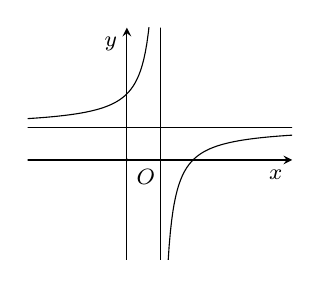
\begin{tikzpicture}[>=stealth,line join=round,line cap=round,font=\footnotesize,scale=.6]
            \begin{scope}[xscale=0.7,yscale=0.7]
                \clip(-3,-3)rectangle (5,4);
                \draw[->] (-4,0)--(5,0) node[below left]{$x$};
                \draw[->] (0,-4)--(0,4)node[ below left]{$y$} ;
                \draw[domain=-4:0.8,samples=100] plot (\x,{(\x-2)/(\x-1)});
                \draw[domain=1.2:5,samples=100] plot (\x,{(\x-2)/(\x-1)});
                \draw[line width=.02] (-4,1)--(5.3,1);
                \draw[line width=.02] (1,-4)--(1,4) ;
                \fill(0,0)circle (0.05)node[below right]{$O$};
            \end{scope}
    \end{tikzpicture}}
    \loigiai{Hàm số xác định khi và chỉ $x\ne 1$.
        Từ đồ thị hàm số suy ra	 \[\displaystyle\lim\limits_{x\to 1^+}\dfrac{x+a}{x-1}=-\infty,\]
        kéo theo $a+1<0$.\\
        Vậy $y'=-\dfrac{a+1}{(x-1)^2}>0$ với mọi $x\ne 1$.
    }
\end{ex}
\begin{ex}%[2D1B5-1]
    Cho hàm số $y=ax^3+bx^2+cx+d$ có đồ thị như hình vẽ. Mệnh đề nào sau đây đúng
    \begin{center}
        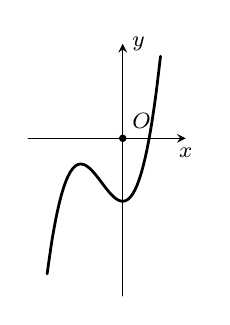
\begin{tikzpicture}[>=stealth,line join=round,line cap=round,font=\footnotesize,scale=.4]
            %	\draw[step=1,gray,very thin]
            %	(-3,-3.3) grid (0.5,3.1);
            \draw[->] (-3,0) --(0,0) node[above
            right]{$O$} -- (2,0)
            node[below]{$x$};
            \draw[->](0,-5)--(0,3)
            node[right]{$y$};
            \draw[smooth,black,line width=1]
            plot[domain=-2.4:1.2]
            (\x,{(\x)^3+2*(\x)^2-2});
            \fill [black, draw=black, line width=0.4pt] (0,0) circle (0.1cm) ;
        \end{tikzpicture}
    \end{center}
    \choice
    { $a>0;b<0;c=0;d<0$}
    {$a>0;b=0;c>0;d<0$}
    { \True $a>0;b>0;c=0;d<0$}
    {$a>0;b=0;c<0;d<0$}
    \loigiai{Dựa vào đồ thị hàm số ta thấy đây là hàm bậc $3$ và $a>0$.\\
        Hàm số cắt trục tung tại điểm có tung độ âm nên $d<0$.\\
        Hàm số đạt cực trị tại $x=0$ do đó $c=0$.\\
        Lúc này $y'=3ax^2+2bx$, gọi $x_{1}$, $x_{2}$ là 2 điểm cực trị.\\
        Dựa vào đồ thị và $y'$ ta có $x_{1}+x_{2}=-\dfrac{2b}{3a}<0$. Do đó $b>0$.
    }
\end{ex}
\begin{ex}%[2D1B5-4]
    Tọa độ các giao điểm của đồ thị hàm số $y=\dfrac{x-1}{x+1}$ và đường thẳng $y=x-1$ là:
    \choice
    {$(-1;0)$, $(0;1)$}
    {$(-1;0)$, $(0;-1)$}
    {$(1;0)$}
    {\True $(1;0)$, $(0;-1)$}
    \loigiai{
        Phương trình hoành độ giao điểm của đồ thị hàm số $y=\dfrac{x-1}{x+1}$ và đường thẳng $y=x-1$ là:
        \[\dfrac{x-1}{x+1}=x-1\Leftrightarrow \heva{& x\ne -1 \\& x^2-x=0}\Leftrightarrow \hoac{& x=0 \\& x=1}\]
        Với $x=0\Rightarrow y=-1$.\\
        Với $x=1\Rightarrow y=0$.
    }
\end{ex}
\begin{ex}%[2D1B5-1]
    \immini
    {Đồ thị sau đây là đồ thị của hàm số nào?
        \choice
        {$y = x^4-3x^2-1$}
        {$y = x^4-2x^2-1$}
        {$y=\dfrac{-1}{4}x^4+3x^2-1$}
        {\True $y = x^4+2x^2-1$}
    }
    {
        % Đồ thị hàm y=ax^4+bx^2+c. Nếu hệ số lớn cần điều chỉnh hệ trục, vùng lưới, domain và lệnh \clip
        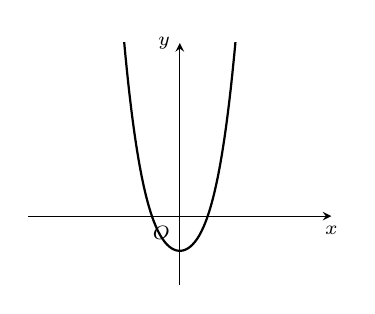
\begin{tikzpicture}[>=stealth,x=1cm,y=0.8cm,scale=0.55]
            \def\a{1} % Hệ số a phải khác 0
            \def\b{2}
            \def\c{-1}
            %\draw[color=gray,dash pattern=on 1pt off 1pt,xstep=1.0cm,ystep=1.0cm] (-5.2,-5.2) grid (5.2,5.2);
            \draw[->] (-3.5,0) -- (3.5,0) node[below] {\scriptsize $x$};
            \draw[->] (0,-2) -- (0,5) node[left] {\scriptsize $y$};
            \draw (0,0)node[below left]{\scriptsize $O$};
            \clip (-3.5,-2)rectangle(3.5,5);
            \draw[thick,samples=150,smooth,domain=-4:4] plot(\x,{\a*(\x)^4+(\b)*(\x)^2+(\c)});
        \end{tikzpicture}
    }
    \loigiai{
        Dựa vào các đáp án và đồ thị thì hàm số
        có dạng $y = ax^4+bx^2+d \,(a\neq 0)$.\\
        Vì đồ thị đi lên theo chiều từ trái qua phải nên $ a>0 $.\\
        Suy ra loại đáp án $ C $.
        Vì đồ thị hàm số có $ 1 $ cực trị nên $ ab\ge0 $.\\
        Suy ra loại đáp án $ A $ và $ B $.
    }
\end{ex}
\begin{ex}%[2D1K5-1]
    \immini{Cho hàm số $f(x)=\dfrac{ax-2}{bx+c}$ với có bảng biến thiên như hình vẽ bên. Giá trị $a+b+c$ thuộc khoảng nào dưới đây?
        \choice
        {\True $\left(-1;1\right)$}
        {$\left(-2;-1\right)$}
        {$\left(2;3\right)$}
        {$\left(1;+\infty\right)$}}
    {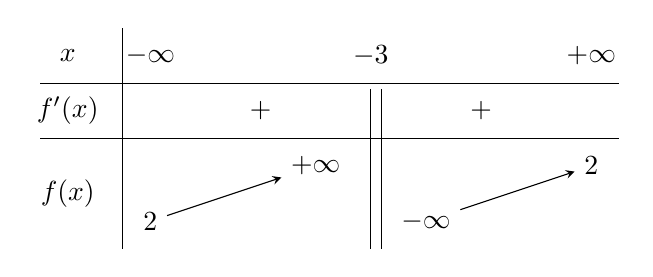
\begin{tikzpicture}[scale=0.7]
            \foreach \gt[count=\i from 0] in {-\infty,-3,+\infty}\path (4*\i,0) node{$\gt$};
            \foreach \gt[count=\i from 0] in {+,+} \path (4*\i+2,-1) node{$\gt$};
            \foreach \x/\y/\gt in {-1.5/0/x,-1.5/-1/f'(x),-1.5/-2.5/f(x), 0/-3/2, 3/-2/+\infty, 5/-3/-\infty,8/-2/2}\path (\x,\y) node(\x){$\gt$};
            \draw (-2,-.5)--(8.5,-.5) (-2,-1.5)--(8.5,-1.5) (-.5,.5)--(-.5,-3.5) (4,-0.6)--(4,-3.5) (4.2,-0.6)--(4.2,-3.5);
            \foreach \x/\y in {0/3,5/8}\draw[-stealth] (\x)--(\y);
        \end{tikzpicture}
    }
    \loigiai{
        Dựa vào bảng biến thiên ta có:
        \begin{itemize}
            \item $\lim\limits_{x\to\pm\infty}f(x)=2\Rightarrow y=2$ là tiệm cận ngang của đồ thị hàm số $\Rightarrow\dfrac{a}{b}=2\Rightarrow a=2b$.
            \item $\lim\limits_{x\to{3^+}}f(x)=-\infty\Rightarrow x=3$ là tiệm cận đứng của đồ thị hàm số $\Rightarrow\dfrac{-c}{b}=3\Rightarrow c=-3b$.
            \item Hàm số đồng biến trên các khoảng $\left(-\infty ;3\right)$ và $\left(3;+\infty\right)$ nên suy ra $f'(x) > 0\Rightarrow ac+2b > 0$
            $$\Leftrightarrow-6b^2+2b > 0\Leftrightarrow 0 < b <\dfrac{1}{3}\Rightarrow \heva{&0<a<\dfrac{2}{3}\\&-1<c<0}\Rightarrow-1 < a+b+c < 1.$$
        \end{itemize}
    }
\end{ex}
\begin{ex}%[2D1K5-1]
    \immini{Cho hàm số $y=\dfrac{ax-b}{x-1}$ có đồ thị như hình vẽ bên dưới. Khẳng định nào sau đây là đúng?
        \choice
        {\True $ b<a<0 $}
        {$ 0<b<a $}
        {$ b<0<a $}
        {$ 0<a<b $}
    }{
        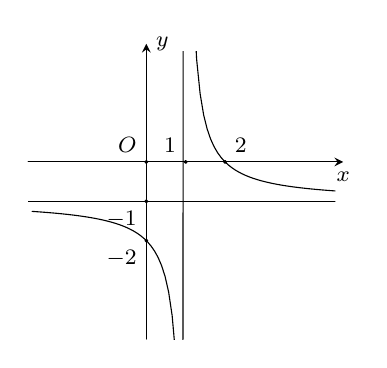
\begin{tikzpicture}[scale=0.5, font=\footnotesize, line join=round, line cap=round, >=stealth]
            \draw[->] (-3,0)--(0,0) node[above left]{$O$}--(5,0) node[below]{$x$};
            \draw[->] (0,-4.5) --(0,3) node[right]{$y$};
            \clip (-3.0,-4.5) rectangle (4.8,2.8);
            \draw [domain=-2.9:5.9, samples=100] %
            plot (\x, {(-1*(\x)+2)/(\x-1)});
            %\draw [line width = 1pt] (1,-5)--(1,3); %TCD
            \draw (-3,-1)--(6,-1); %TCN
            \draw [fill=black]
            (0,0) circle (1pt)
            (1,0) node[above left]{$1$} circle (1pt)
            (2,0) node[above right]{$2$} circle (1pt)
            (0,-1) node[below left]{$-1$} circle (1pt)
            (0,-2) node[below left]{$-2$} circle (1pt);
        \end{tikzpicture}
    }
    \loigiai{
        Tập xác định $\mathscr{D}=\mathbb{R}\setminus\{1\}$.\\
        Ta có $y'=\dfrac{b-a}{(x-1)^2}$.\\
        Vì hàm số nghịch biến nên $b-a<0\Leftrightarrow b<a$.\\
        Từ đồ thị ta có $x=0, y=-2$ và $x=2, y=0$ nên ta được $\heva{&b=-2\\&2a-b=0}\Rightarrow a<0$.\\
        Vậy $b<a<0$.
    }
\end{ex}
\begin{ex}%[2D1Y5-1]
    \immini
    {
        Hình vẽ bên là đồ thị của hàm số nào dưới đây?
        \choice
        {$y=-x^2+x-1$}
        {$y=x^4-x^2+1$}
        {\True $y=x^3-3x+1$}
        {$y=-x^3-3x+1$}
    }
    {
        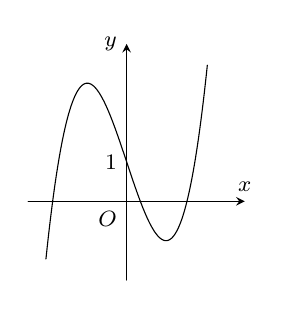
\begin{tikzpicture}[scale=0.5, font=\footnotesize, line join=round, line cap=round, >=stealth]
            \draw[->](-2.5,0)--(3,0)node[above]{$x$};
            \draw[->](0,-2)--(0,4)node[left]{$y$};
            \draw[smooth, samples=150, domain=-2.05:2.05]plot(\x,{((\x)^3-3*(\x)+1)});
            \draw(0,0)node[below left]{$O$};
            \draw(0,1)node[left]{$1$};
        \end{tikzpicture}
    }
    \loigiai
    {
        Dựa vào đồ thị ta có hàm số cần tìm là hàm số bậc ba $y=ax^3+bx^2+cx+d$. \\
        Ta có $\lim\limits_{x\to+\infty} y=+\infty$ nên hệ số $a>0$. \\
        Đồ thị hàm số cắt $Oy$ tại $A(0;1)$ nên $d=1$. \\
        Vậy đồ thị đã cho là của hàm số $y=x^3-3x+1$.
    }
\end{ex}
\begin{ex}%[2D1Y5-1]
    \immini{Đường cong ở hình bên là đồ thị của hàm số $y=ax^3+b x^2+cx+d$. Mệnh đề nào sau đây đúng?
        \choice
        {$y'=0$ có 3 nghiệm và $a<0$}
        {$y'=0$ có 2 nghiệm và $a>0$}
        {$y'=0$ có 3 nghiệm và $a>0$}
        {\True $y'=0$ có 2 nghiệm và $a<0$}}{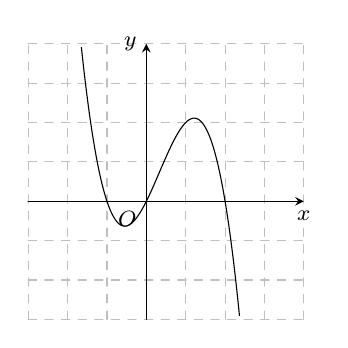
\begin{tikzpicture}[scale=0.5,>=stealth, font=\footnotesize, line join=round, line cap=round]
            \def\a{0.6} \def\b{-3.51} \def\c{6.8} \def\d{-4.35} % Hệ số
            \def\xmin{-3} \def\xmax{4}
            \def\ymin{-3} \def\ymax{4}
            \draw[color=gray!50,dashed] (\xmin,\ymin) grid (\xmax,\ymax);
            \draw[->] (\xmin,0)--(\xmax,0) node [below]{$x$};
            \draw[->] (0,\ymin)--(0,\ymax) node [left]{$y$};
            \node at (0,0) [below left]{$O$};
            \clip (\xmin+0.1,\ymin+0.1) rectangle (\xmax-0.5,\ymax-0.1);
            \draw[smooth,samples=300] plot(\x,{-1*(\x+1)*(\x)*(\x-2)});
    \end{tikzpicture}}
    \loigiai{
        Dựa vào hình dáng đồ thị ta có $y'=0$ có 2 nghiệm và $a<0$.
    }
\end{ex}
\begin{ex}%[2D1B5-3]
    Tìm tất cả giá trị thực của tham số $m$ để phương trình $x^4-2x^2-m+3=0$ có hai nghiệm phân biệt.
    \choice
    {$m>3$}
    {$m\ge 3$}
    {\True $m>3$ hoặc $m=2$}
    {$m=2$ hoặc $m=3$}
    \loigiai{$x^4-2x^2-m+3=0\Leftrightarrow m=x^4-2x^2+3$.\\
        Xét $f(x)=x^4-2x^2+3$, $\mathscr{D}=\mathbb{R}$.\\
        $f'(x)=4x^3-4x$, $f'(x)=0\Leftrightarrow \hoac{&x=0\\&x=1\\&x=-1.}$\\
        Bảng biến thiên
        \begin{center}
            
\begin{tikzpicture}[>=stealth]
                \tkzTabInit[nocadre=false,lgt=1.2,espcl=2.2,deltacl=0.5]{$x$/.7 ,$f'(x)$/.7,$f(x)$/2}
                {$-\infty$ , $-1$ , $0$ , $1$ , $+\infty$}
                \tkzTabLine{ , - , $0$ , + , $0$ , - , $0$ , + , }
                \tkzTabVar{+/$+\infty$ , -/$2$, +/$3$ , -/$2$ , +/$+\infty$}
            \end{tikzpicture}
        \end{center}
        YCBT $\Leftrightarrow \hoac{&m=2\\&m>3.}$
    }
\end{ex}
\begin{ex}%[2D1B5-1]
    \immini{Giả sử đồ thị hình bên là của một trong các hàm được liệt kê ở các đáp án A, B, C, D. Hỏi đó là hàm số nào?
        \choice
        {\True $y=x^4-2x^2-1$}
        {$y=x^4+2x^2$}
        {$y=x^4-2x^2+1$}
        {$y=x^4-2x^2$}
    }
    {
        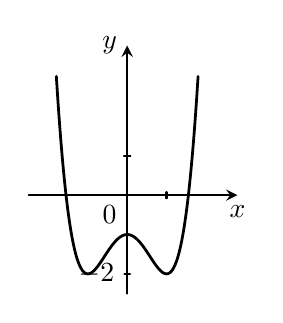
\begin{tikzpicture}[line cap=round,line join=round,>=stealth, scale=0.5, thick]
            \tkzInit[xmax=3,xmin=-2.5,ymax=4,ymin=-1.5]
            \draw[->,>=stealth] (-2.5,0)--(2.8,0) node[below]{$x$};
            \draw[->,>=stealth] (0,-2.5) --(0,3.8) node[left]{$y$};
            \draw[line width=1pt,smooth,samples=100,domain=-1.8:1.8] plot(\x,{(\x)^(4)-2*(\x)^(2)-1});
            \foreach \x in { , , , }
            \draw[shift={(\x,0)},color=black] (0pt,2pt) -- (0pt,-2pt) node[below] { $\x$};
            \foreach \y in {-2,, , , , }
            \draw[shift={(0,\y)},color=black] (2pt,0pt) -- (-2pt,0pt) node[left] {\normalsize $\y$};
            \node[below left] at (-0.01,0) {$0$};
        \end{tikzpicture}
    }
    \loigiai{
        Đồ thị hàm số cắt $Oy$ tại $A(0;-1)$ nên chọn phương án $y=x^4-2x^2-1$.
    }
\end{ex}
\begin{ex}%[2D1B5-4]
    Tìm giá trị thực của tham số $m$ để đường thẳng $d\colon y=(2m-1)x+m+3$ song song với đường thẳng đi qua các điểm cực trị của đồ thị hàm số $y=x^3-3x^2+1$.
    \choice
    {$m=\dfrac{1}{2}$}
    {$m=-\dfrac{3}{4}$}
    { $m=\dfrac{3}{4}$}
    {\True $m=-\dfrac{1}{2}$}
    \loigiai{
        Xét hàm số $y=f(x)=x^3-3x^2+1$.\\
        $f'(x)=3x^2-6x$; $f'(x)=0\Leftrightarrow \hoac{&x=0 \\&x=2. }$\\
        Với $x=0\Rightarrow y=1$; $x=2\Rightarrow y=-3$.\\
        Đường thẳng đi qua $(0;1)$ và $(2;-3)$ là $\Delta\colon y=-2x+1$.\\
        Do $d\parallel\Delta\Leftrightarrow\heva{&2m-1=-2 \\&m+3\ne 1 }\Leftrightarrow\heva{&m=-\dfrac{1}{2} \\&m\ne -3 }\Leftrightarrow m=-\dfrac{1}{2}$.
    }
\end{ex}
\begin{ex}%[2D1K5-1]
    Cho đồ thị hàm số $y=\dfrac{ax+b}{x-c}$ như hình vẽ. Tìm khẳng định
    \textbf{đúng}?
    \begin{center}
        \begin{tikzpicture}[>=stealth,scale=0.3, line join=round, line
            cap=round,font=\footnotesize]
            \draw[->] (-7,0)--(5,0) node [below]{$x$};
            \draw[->] (0,-4)--(0,8) node [left]{$y$};
            \draw[fill=black] (0,0) circle (2pt) node[below left]{$O$};
            \draw[smooth,samples=300,domain=-7:-1.5] plot(\x,{(2*\x-1)/(\x+1)});
            \draw[smooth,samples=300,domain=-0.5:5] plot(\x,{(2*\x-1)/(\x+1)});
            \draw[dashed] (-7,2)--(5,2);
            \draw[dashed] (-1,-4)--(-1,8);
        \end{tikzpicture}
    \end{center}
    \choice
    {$a<0$, $b>0$, $c>0$ }
    {$a>0$, $b<0$, $c>0$ }
    {\True $a>0$, $b>0$, $c<0$ }
    {$a>0$, $b<0$, $c<0$}
    \loigiai{
        Hàm số có dạng $y=\dfrac{ax+b}{x-c}$.
        \begin{itemize}
            \item Tiệm cận ngang $y=y_0>0 \Rightarrow a>0$.
            \item Tiệm cận đứng $x=x_0<0 \Rightarrow c<0$.
            \item Hàm số nghịch biến nên $-ac-b<0$
        \end{itemize}
        Suy ra $a>0$, $b>0$, $c<0$.
    }
\end{ex}
\begin{ex}%[2D1B5-3]
    \immini{Cho hàm số $y=f(x)$ có đồ thị như hình vẽ. Số nghiệm của phương trình $2f^2(x)-1=0$ trên đoạn $[-2;3]$ là
        \choice
        {$7$}
        {\True $8$}
        {$5$}
        {$4$}
    }{
        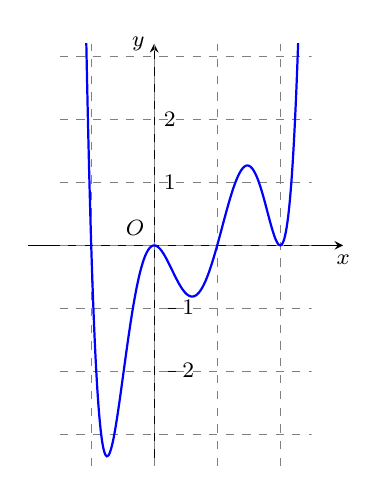
\begin{tikzpicture}[>=stealth,x=1cm,y=1cm,scale=0.8,font=\footnotesize]
            \draw[->] (-2,0) -- (3,0) node[below] {$x$};
            \draw[->] (0,-3.5) -- (0,3.2) node[left] {$y$};
            \foreach \y in {-2,-1,1,2} {\draw (0,\y)node[right]{$\y$};}
            \draw (0,0)node[above left]{$O$};
            \clip (-1.5,-3.5)rectangle(2.5,3.2);
            \draw[dashed,gray] (-1.5,-3.5)grid(2.5,3.2);
            \draw[thick,blue,samples=150,smooth,domain=-1.2:2.5] plot(\x,{1.8*((\x)+1)*(\x)^2*((\x)-1)*((\x)-2)^2});
        \end{tikzpicture}
    }
    \loigiai{
        Ta có: $2f^2(x)-1=0 \Leftrightarrow f^2(x)=\dfrac{1}{2} \Leftrightarrow \hoac{& f(x)=\dfrac{1}{\sqrt{2}} \\& f(x)=-\dfrac{1}{\sqrt{2}}.}$\\
        Dựa vào đồ thị ta thấy:
        \begin{itemize}
            \item Đường thẳng $y=\dfrac{1}{\sqrt{2}}$ cắt đồ thị hàm số $y=f(x)$ tại $4$ điểm. Do đó phương trình $f(x)=\dfrac{1}{\sqrt{2}}$ có $4$ nghiệm.
            \item Đường thẳng $y=-\dfrac{1}{\sqrt{2}}$ cắt đồ thị hàm số $y=f(x)$ tại $4$ điểm. Do đó phương trình $f(x)=-\dfrac{1}{\sqrt{2}}$ có $4$ nghiệm.
        \end{itemize}
        Vậy phương trình $2f^2(x)-1=0$ có $8$ nghiệm
    }
\end{ex}
\begin{ex}%[2D1B5-4]
    Cho hàm số $y=g(x)$ có tập xác định là $(0;+\infty)$ và có bảng biến thiên như sau
    \begin{center}
        
\begin{tikzpicture}
            \tkzTabInit[nocadre=false,lgt=1.2,espcl=2.5,deltacl=0.6]
            {$x$/1,$g’(x)$/1,$g(x)$/2}
            {$0$,$+\infty$}
            \tkzTabLine{ ,+, }
            \tkzTabVar{-/$0$,+/$+\infty$}
        \end{tikzpicture}
    \end{center}
    Tìm số giao điểm của đồ thị hàm số $y=f(x)=x-\dfrac{1}{3}-x^2$ và $y=g(x)$.
    \choice
    {\True $0$}
    {$1$}
    {$3$}
    {$2$}
    \loigiai{
        Ta có, 	$f'(x)=1-2x$; $f'(x)=0$ $\Leftrightarrow x=\dfrac{1}{2}$.
        \begin{center}
            
\begin{tikzpicture}
                \tkzTabInit[nocadre=false,lgt=1.2,espcl=2.5,deltacl=0.6]
                {$x$ /1,$f'(x)$ /0.8,$f(x)$/2}
                {$0$,$\dfrac{1}{2}$,$+\infty$}
                \tkzTabLine{,+,$0$,-,}
                \tkzTabVar{-/$-\dfrac{1}{3}$, +/$-\dfrac{1}{12}$,-/$-\infty$}
            \end{tikzpicture}
        \end{center}
        Ta có, xét trên $(0;+\infty)$ thì $g(x)>0$ và $f(x)<0$ nên số giao điểm của hai đồ thì hàm số $y=f(x)$ và $y=g(x)$ bằng $0$.
    }
\end{ex}
\begin{ex}%[2D1B5-3]
    Cho hàm số $y=f(x)$ có đồ thị như hình. Tìm số nghiệm của phương trình $4f(x)-3=0$.
    \begin{center}
        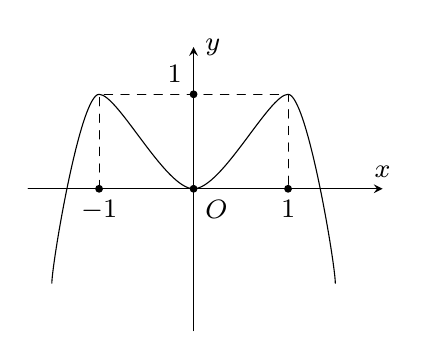
\begin{tikzpicture}[line join=round, line cap = round, >=stealth, scale=1.2,font=\footnotesize,transform shape]
            \draw[->] (-1.75,0) -- (2,0)node[above]{$x$};
            \draw[->] (0,-1.5) -- (0,1.5)node[right]{$y$};
            %\draw[-] (-1.5,0.75) -- (1.5,0.75) node[right]{$y=\frac{3}{4}$};
            \draw[fill=black]
            (0,0) circle(1pt) node[below right]{$O$}
            (-1,0) circle(1pt) node[below]{$-1$}
            (1,0) circle(1pt) node[below]{$1$}
            (0,1) circle(1pt) node[above left]{$1$}
            ;
            \draw[dashed] (-1,0)--(-1,1)--(1,1)--(1,0);
            \draw
            (-1.5,-1) .. controls +(90:.2) and +(180:.2) .. (-1,1)
            .. controls +(0:.2) and +(180:.3) .. (0,0)
            .. controls +(0:.3) and +(180:.2) .. (1,1)
            .. controls +(0:.2) and +(90:.2) .. (1.5,-1)
            ;
        \end{tikzpicture}
    \end{center}
    \choice
    {\True $4$}
    {$3$}
    {$2$}
    {$0$}
    \loigiai{
        Ta có $4f(x)-3=0 \Leftrightarrow f(x)=\dfrac{3}{4}.\quad (*)$
        \begin{center}
            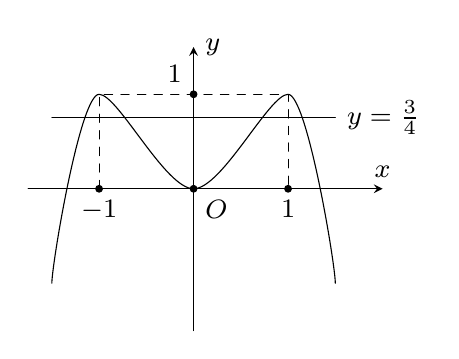
\begin{tikzpicture}[line join=round, line cap = round, >=stealth, scale=1.2,font=\footnotesize,transform shape]
                \draw[->] (-1.75,0) -- (2,0)node[above]{$x$};
                \draw[->] (0,-1.5) -- (0,1.5)node[right]{$y$};
                \draw[-] (-1.5,0.75) -- (1.5,0.75) node[right]{$y=\frac{3}{4}$};
                \draw[fill=black]
                (0,0) circle(1pt) node[below right]{$O$}
                (-1,0) circle(1pt) node[below]{$-1$}
                (1,0) circle(1pt) node[below]{$1$}
                (0,1) circle(1pt) node[above left]{$1$}
                ;
                \draw[dashed] (-1,0)--(-1,1)--(1,1)--(1,0);
                \draw
                (-1.5,-1) .. controls +(90:.2) and +(180:.2) .. (-1,1)
                .. controls +(0:.2) and +(180:.3) .. (0,0)
                .. controls +(0:.3) and +(180:.2) .. (1,1)
                .. controls +(0:.2) and +(90:.2) .. (1.5,-1)
                ;
            \end{tikzpicture}
        \end{center}
        Số nghiệm của phương trình $(*)$ là số giao điểm của đồ thị hàm số $f(x)$ và đường thẳng nằm ngang $y=\dfrac{3}{4}$. \\
        Quan sát hình vẽ, nhận thấy số giao điểm là $4$. Suy ra số nghiệm của phương trình là $4$.
    }
\end{ex}
\begin{ex}%[2D1B5-3]
    Có bao nhiêu giá trị nguyên của tham số $m\in[-2018;2019]$ để đồ thị hàm số $y=x^3-3 mx+3$ và đường thẳng $y=3x+1$ có duy nhất một điểm chung?
    \choice
    {$1$}
    {$2019$}
    {$4038$}
    {\True $2018$}
    \loigiai{
        Xét phương trình hoành độ giao điểm\\
        $x^3-3mx+3=3x+1\Leftrightarrow \dfrac{x^3-3x+2}{3x}=m$ (vì $x=0$ không là nghiệm của phương trình).\\
        Xét hàm số $f(x)=\dfrac{x^3-3x+2}{3x}$ với $x\ne 0$.\\
        $f'(x)=\dfrac{\left(3x^2-3\right)x-\left(x^3-3x+2\right)}{3x^2}=\dfrac{2x^3-2}{3x^2}$, $f'(x)=0\Leftrightarrow x=1$.\\
        Bảng biến thên
        \begin{center}
            
\begin{tikzpicture}
                \tkzTabInit[nocadre=false,lgt=1.2,espcl=2.5,deltacl=0.6]
                {$x$ /0.6, $f'(x)$ /0.6, $f(x)$ /2.1}
                {$-\infty$,$0$,$1$,$+\infty$}
                \tkzTabLine{,-,d,-,$0$,+,}
                \tkzTabVar{+/$+\infty$,-D+/$-\infty$/$+\infty$,-/$0$,+/$+\infty$}
            \end{tikzpicture}
        \end{center}
        Từ bảng biến thiên, suy ra để đồ thị hàm số $y=x^3-3 mx+3$ và đường thẳng $y=3x+1$ có duy nhất một điểm chung thì $m<0$.\\
        Mà $m$ nguyên và $m\in[-2018;2019]$ nên $m\in\{-2018;-2017;\ldots;-1\}$.
    }
\end{ex}
\Closesolutionfile{ans}